%!TEX root = ../main.tex

\chapter{View}
\label{ch:view}


\section{Haupseite und Buchung}

Die Startseite der Anwendung ist in \ref{fig:startseite} dargestellt.
Auf dieser haben Nutzende die Möglichkeit, den Raum zu buchen oder auf andere Ansichten zu wechseln.
Das Banner in allen Ansichten zeigt den aktuellen Raumstatus an.
Insbesondere wird dadurch die Priorität des aktuellen Termins mithilfe der Farbe des Banners angezeigt.

Rechts in dieser Ansicht befindet sich ein Kalender, der die aktuelle Woche und die Termine in diesem Zeitraum anzeigt.
Die Termine sind farblich nach Priorität gekennzeichnet, weitere Informationen können durch Klicken auf den Termin eingesehen werden.
Neben dieser Möglichkeit, den Raum zu buchen, gibt es je nach Anmeldungsstatus einen Anmelde- oder Abmeldebutton und einen separaten Buchungsbutton,
für den die Verwendung des Kalenders Probleme bereitet.
Falls zur Zeit der Verwendung ein Termin des Nutzenden stattfindet, wird ein Quick-Checkout-Button angezeigt,
der es ermöglicht, den Raum schnell freizugeben.
Siehe dazu auch \ref{fig:checkout}.

\begin{figure}[ht]
    \centering
    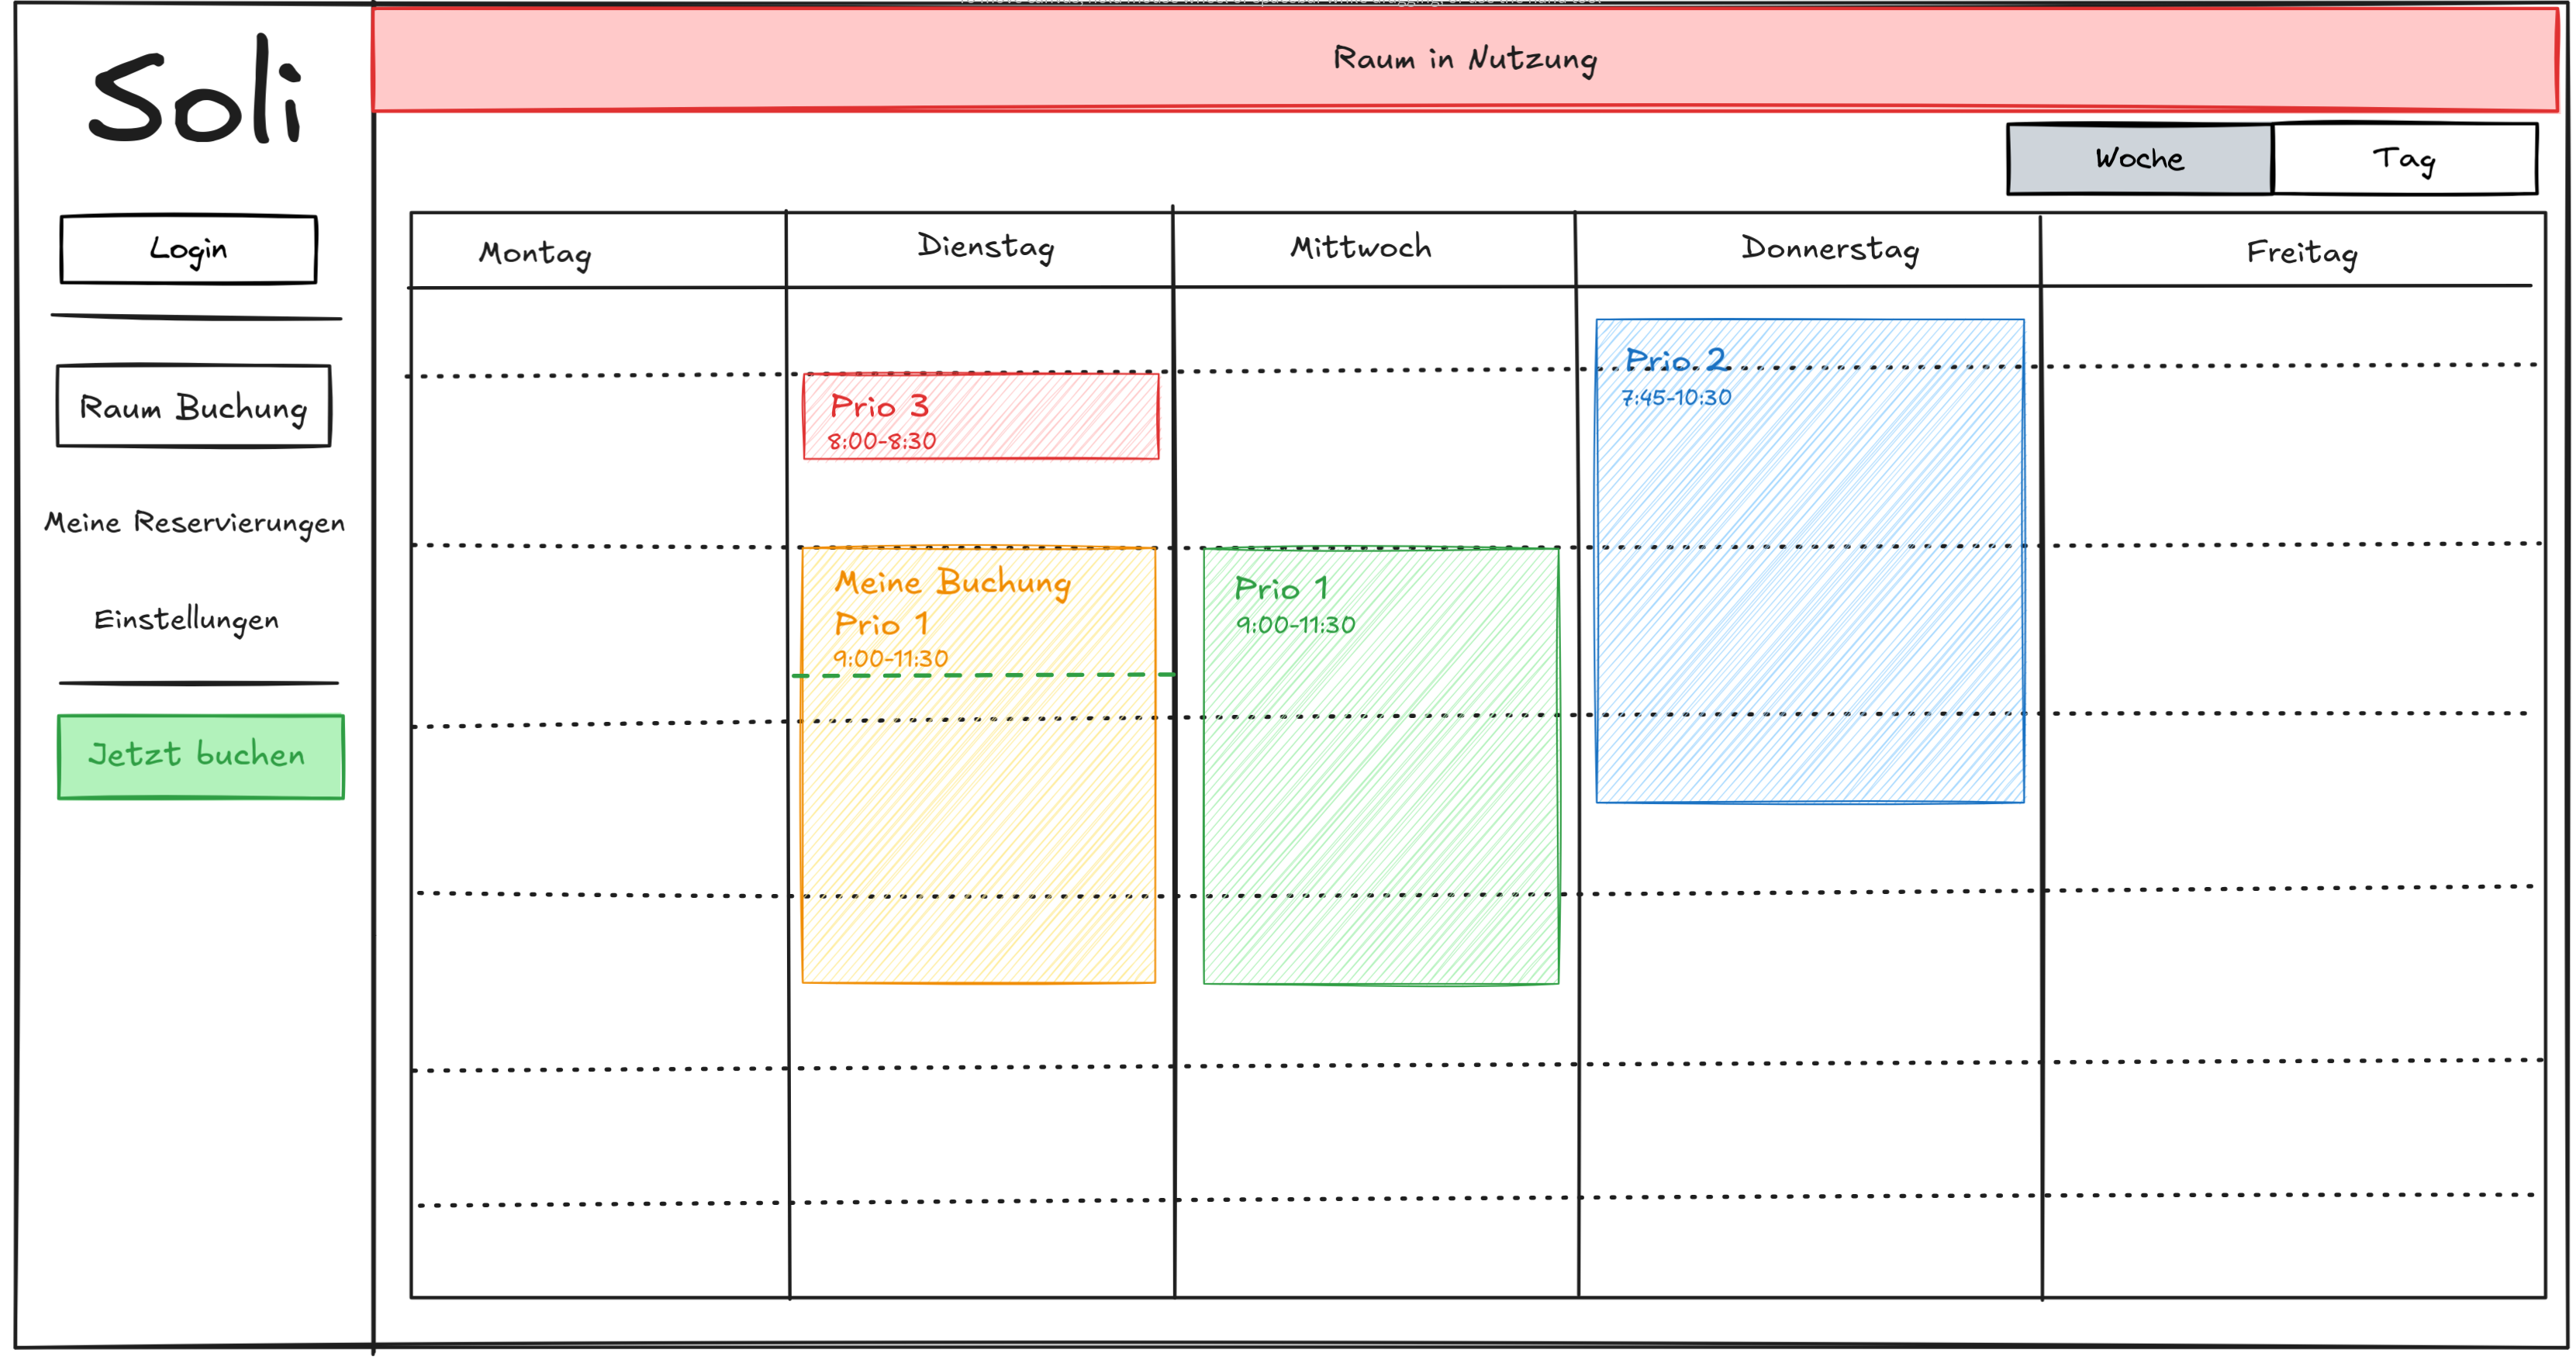
\includegraphics[width=\textwidth]{figures/ui/startseite}
    \caption{Startseite der Anwendung}
    \label{fig:startseite}
\end{figure}
\pagebreak

Sollten Nutzende eine Buchung vornehmen wollen, so klicken diese in den gewünschten Zeitraum
und es wird der Dialog in \ref{fig:buchung} dargestellt.

Der Dialog bietet Nutzenden die Möglichkeit, den genauen Start- und Endzeitpunkt des Termins festzulegen.

Außerdem können Nutzende die Priorität des Termins in Form einer Zahl zwischen 1 und 3 festlegen.
Nutzende können auch angeben, ob sie bereit sind, den Raum mit anderen Nutzenden zu teilen.
Für diesen Zweck werden Ihnen drei Optionen bereitgestellt: \textit{Ja}, \textit{Nein} und \textit{Auf Anfrage}.
Siehe dazu auch \ref{fig:buchung}.

Letztlich können Nutzende eine Beschreibung für den Termin hinterlegen, die anderen angemeldeten Nutzenden angezeigt wird.

\begin{figure}[ht]
    \centering
    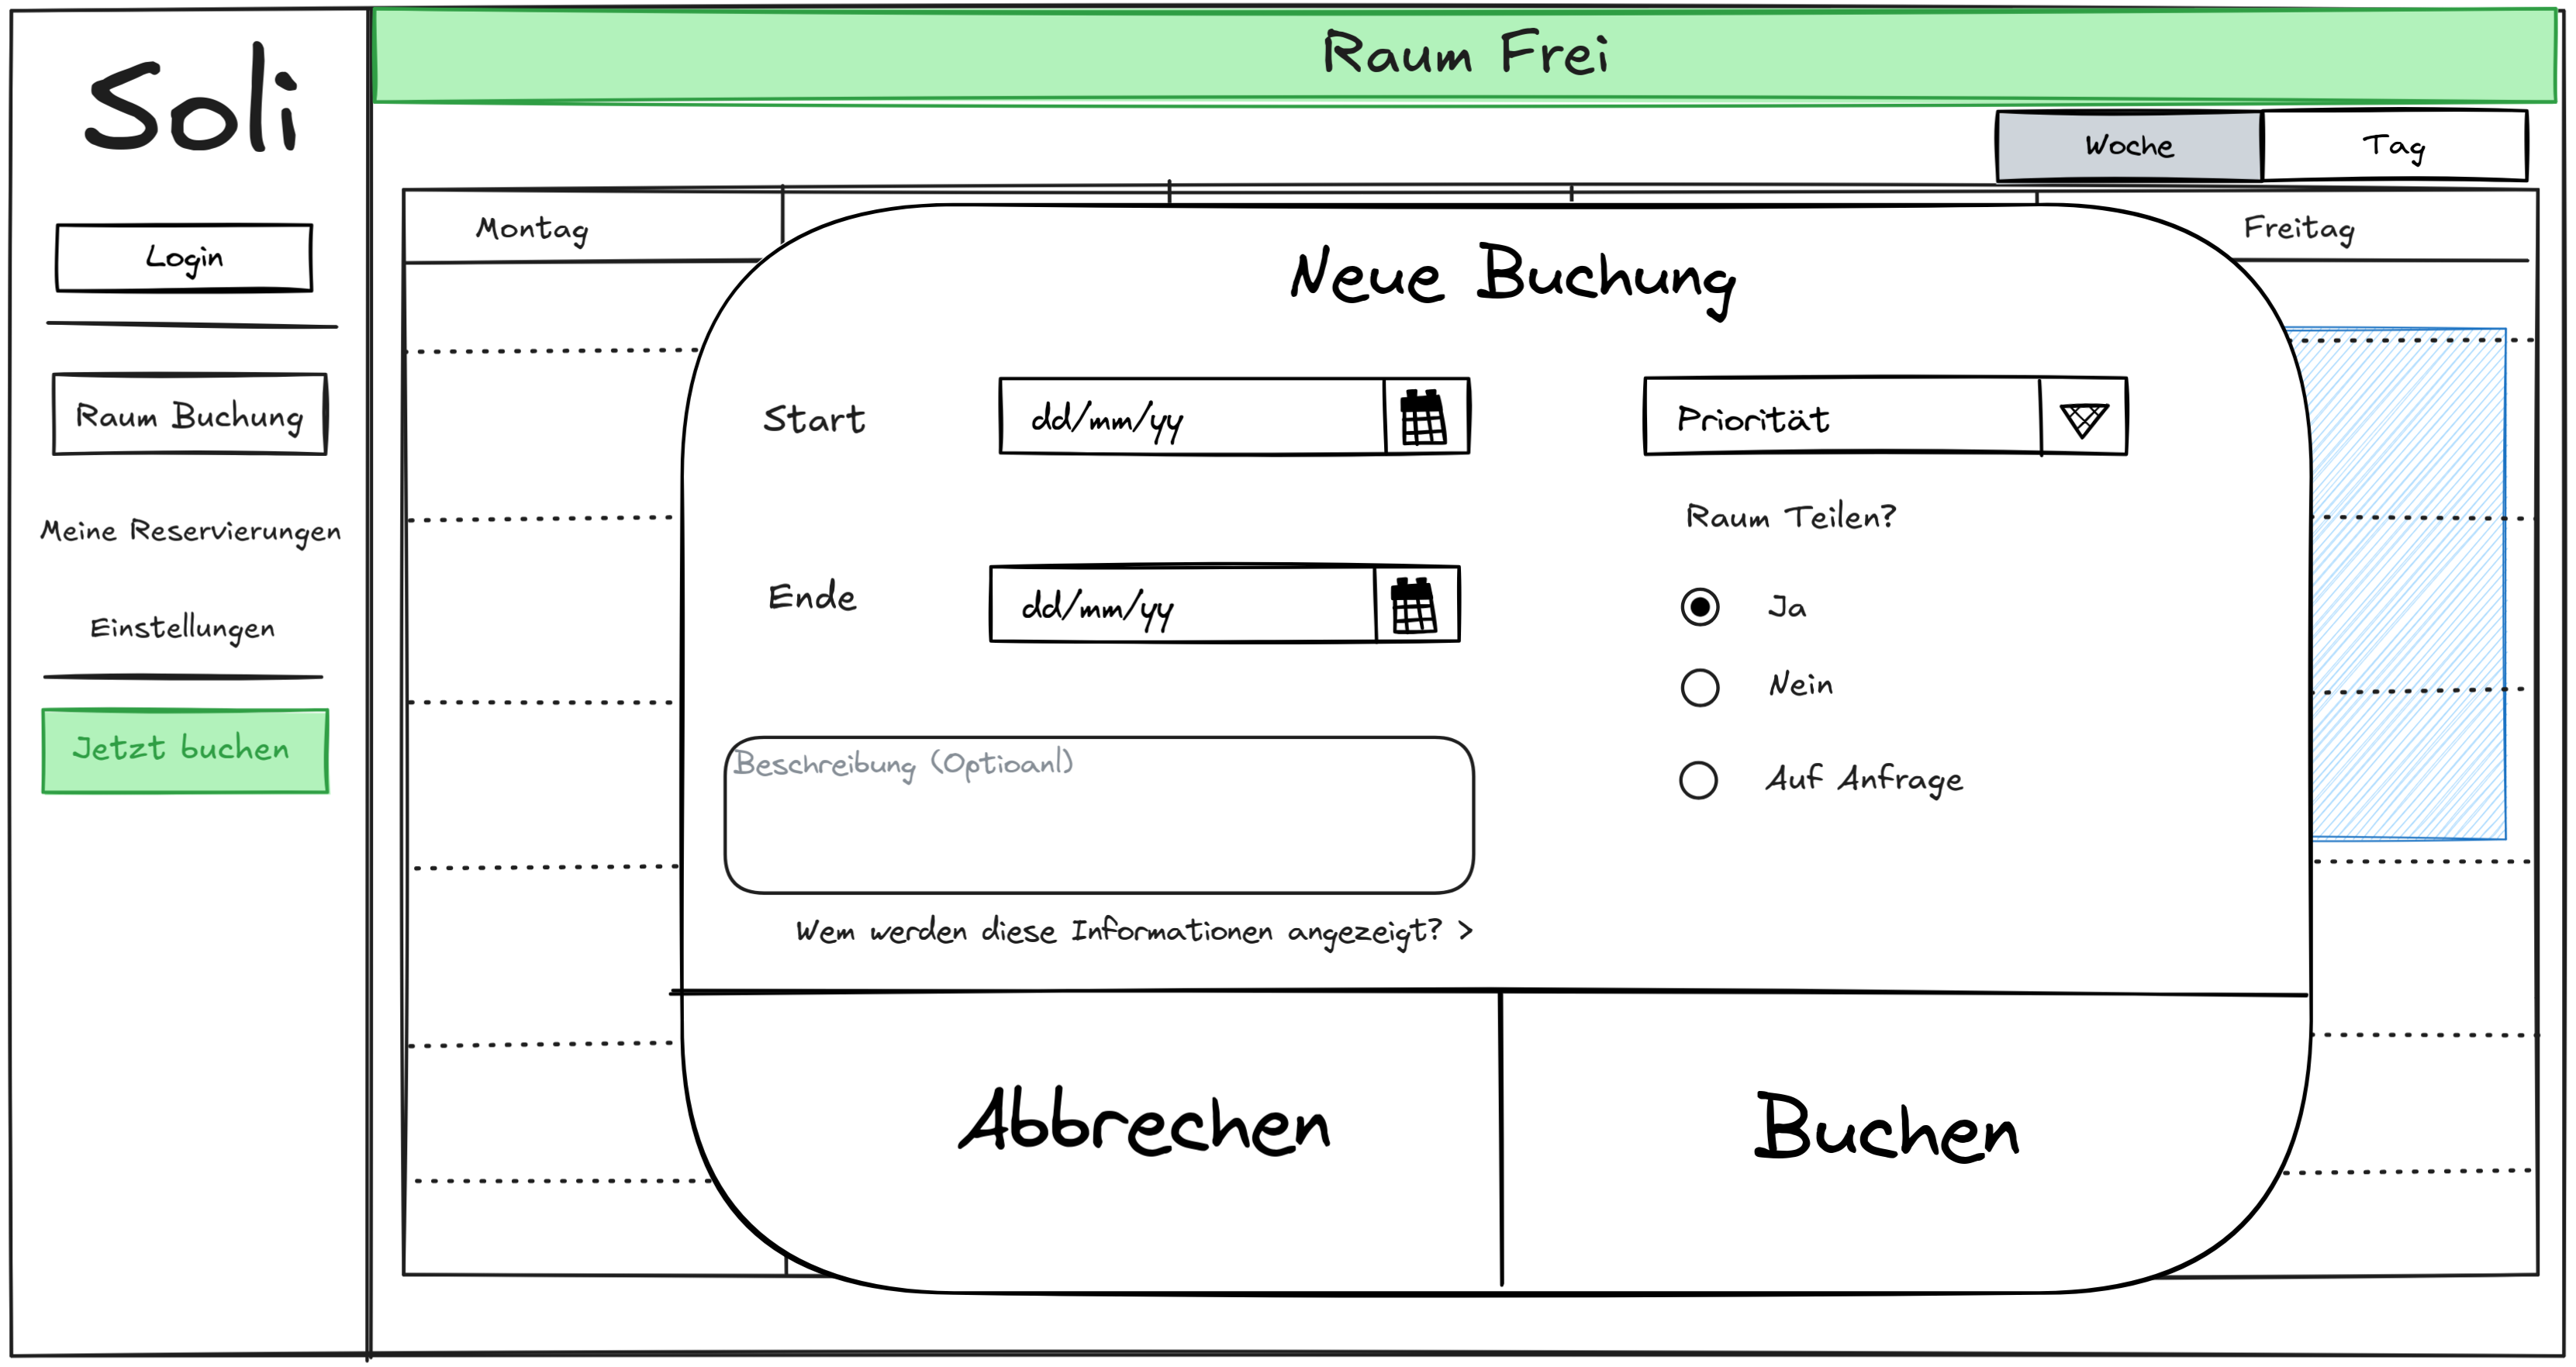
\includegraphics[width=\textwidth]{figures/ui/buchungsdialog}
    \caption{Termin-erstellen}
    \label{fig:buchung}
\end{figure}
\clearpage

Tätigen Nutzende eine Buchung, so werden diese aufgefordert, sich anzumelden.
Der hierzu gehörige Dialog ist in \ref{fig:login} dargestellt.
Alternativ ist dieser Dialog auch über den Anmeldungsbutton, der in Abbildung \ref{fig:startseite} zu sehen ist, erreichbar.

In diesem Dialog wird Nutzenden die Möglichkeit gegeben, sich mit ihrem KIT-Konto, mit einem lokalen Gastkonto oder als Admin anzumelden.

Falls Nutzende die Anmeldung per KIT-Konto wählen, werden sie auf die KIT-Login-Seite weitergeleitet.
Von dort aus können sie sich mit ihren KIT-Zugangsdaten anmelden.

Falls Nutzende die Anmeldung per Gastkonto wählen, werden sie aufgefordert, eine E-Mail-Adresse anzugeben.
Mit der Bestätigung dieser E-Mail-Adresse wird ein temporäres Gastkonto erstellt und die Anmeldung per Cookie gespeichert.

Falls Nutzende die Anmeldung als Admin wählen, werden sie aufgefordert, das Passwort des Adminkontos einzugeben.

Nach einer erfolgreichen Anmeldung werden Nutzende auf die nächste Seite weitergeleitet.

\begin{figure}[ht]
    \centering
    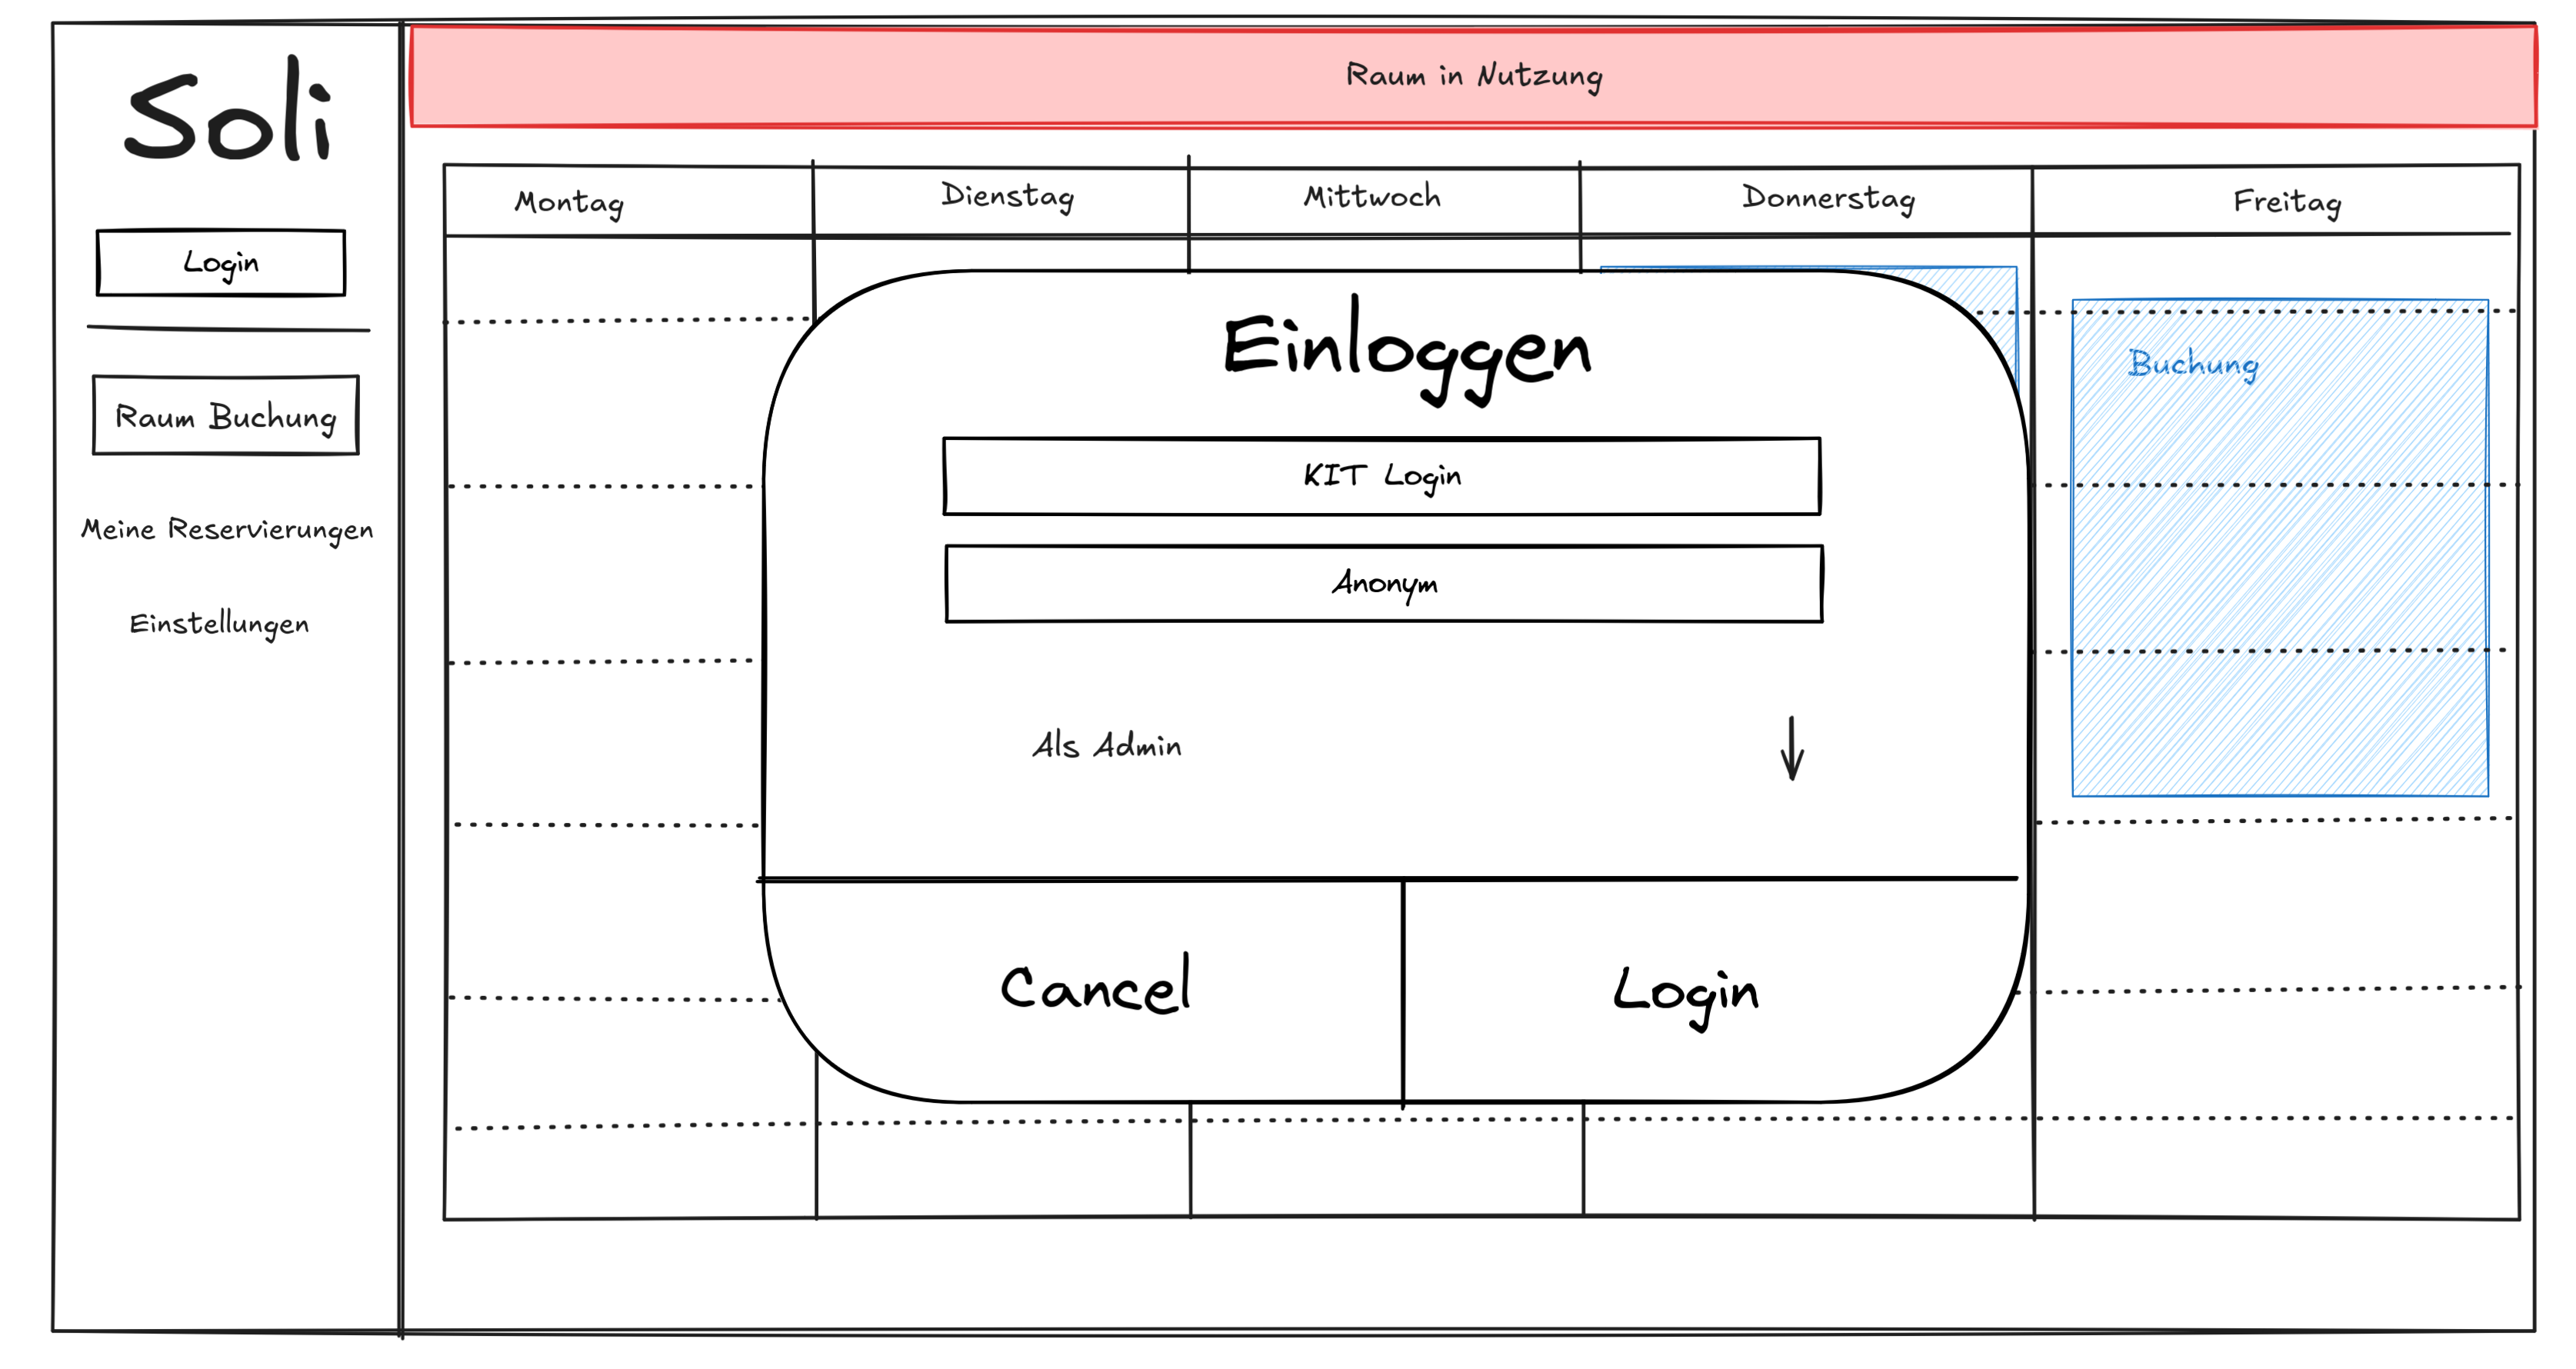
\includegraphics[width=\textwidth]{figures/ui/anmeldungsseite}
    \caption{Anmeldungsseite}
    \label{fig:login}
\end{figure}
\clearpage

Sind Nutzende eingeloggt und belegen den Raum,
so wird ihnen die in Abbildung \ref{fig:checkout} dargestellte Ansicht angezeigt.
Hier können Nutzende den Raum wieder über den Quick-Checkout-Button freigeben.


Ziel dieser Ansicht ist es, Nutzenden das frühe Freigeben des Raumes ohne unnötigen Mehraufwand zu ermöglichen.
\begin{figure}[ht]
    \centering
    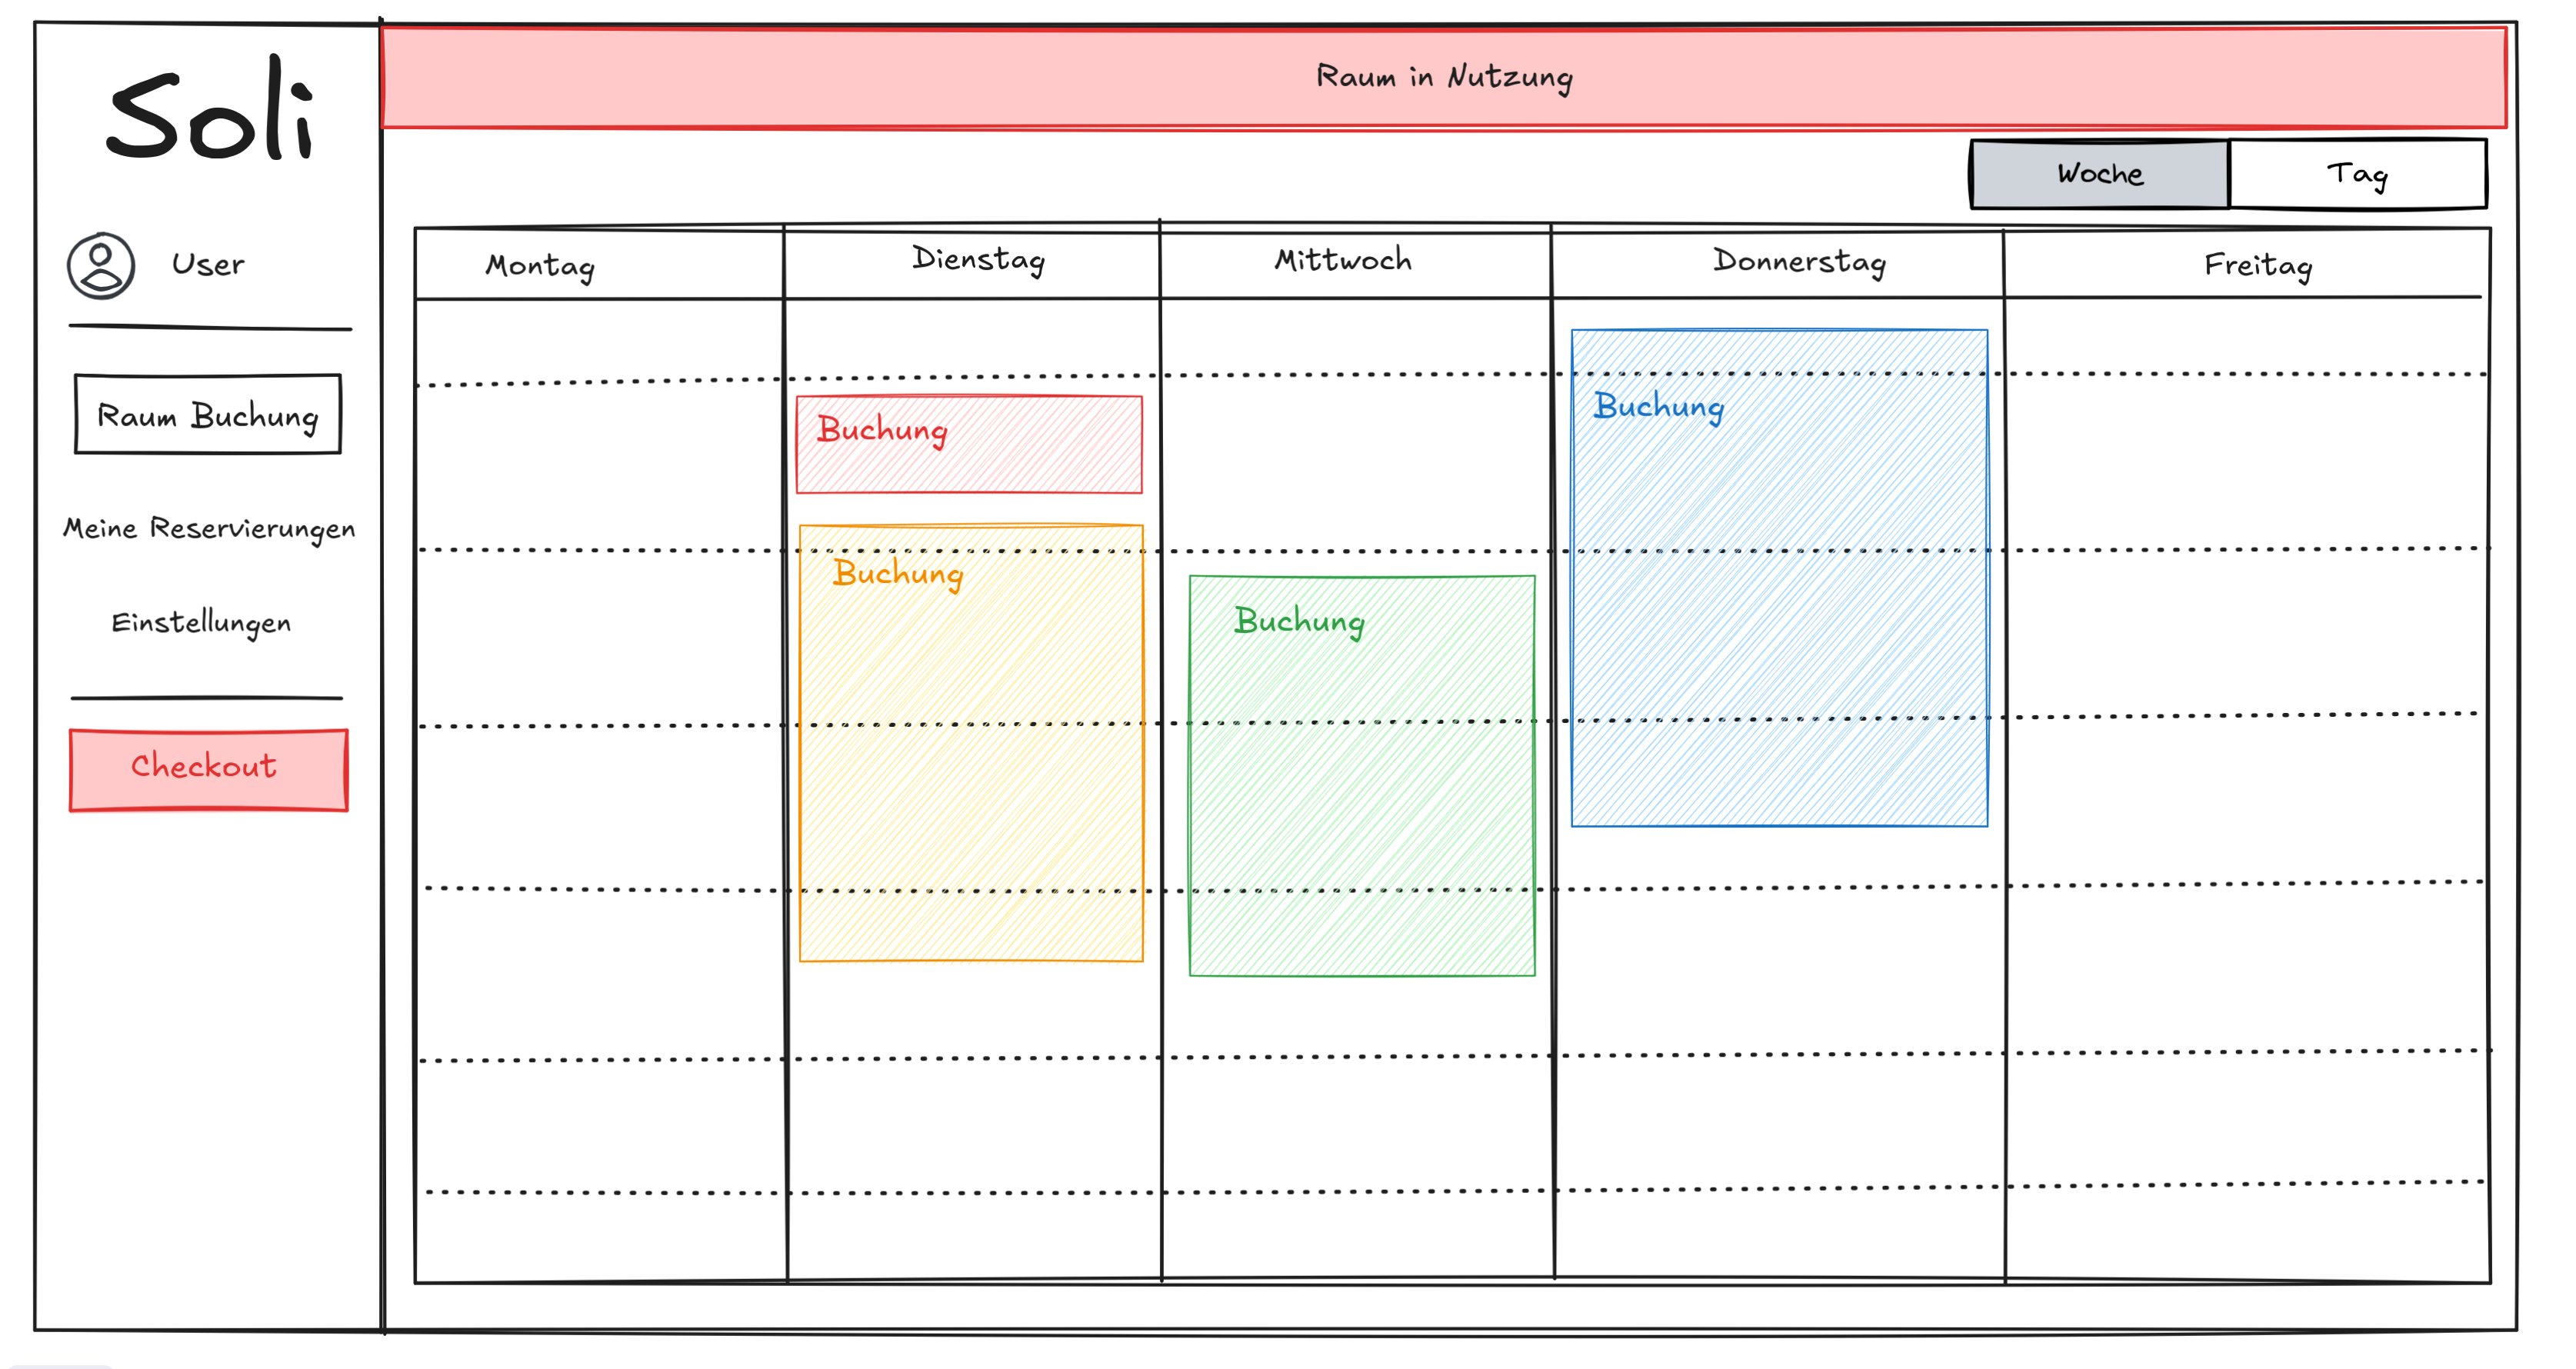
\includegraphics[width=\textwidth]{figures/ui/checkout}
    \caption{Quick Checkout}
    \label{fig:checkout}
\end{figure}
\clearpage

\section{Terminübersicht}
Nutzende, die eine Buchung vorgenommen haben, können diese in der Terminübersicht,
die in Abbildung \ref{fig:overview} dargestellt ist, einsehen und verwalten.

Die Termine in dieser Ansicht werden, anders als in der Ansicht \textit{Kalender}, in Form einer sortierten Liste dargestellt.
Dabei werden die Start- und Endzeitpunkte der Termine, wie auch die Priorität und die Beschreibung angezeigt.

Nutzende haben die Möglichkeit, eine Buchung zu stornieren, indem sie auf den Stornieren-Button klicken.

Außerdem können Nutzende die Ansicht \textit{Termin} (\ref{fig:calendarviewbooking}) zu einem Termin öffnen, indem sie auf den Termin klicken.

\begin{figure}[ht]
    \includegraphics[width=\textwidth]{figures/ui/reservierungsübersicht}
    \caption{Reservierungsübersicht}
    \label{fig:overview}
\end{figure}
\begin{figure}
    \centering
    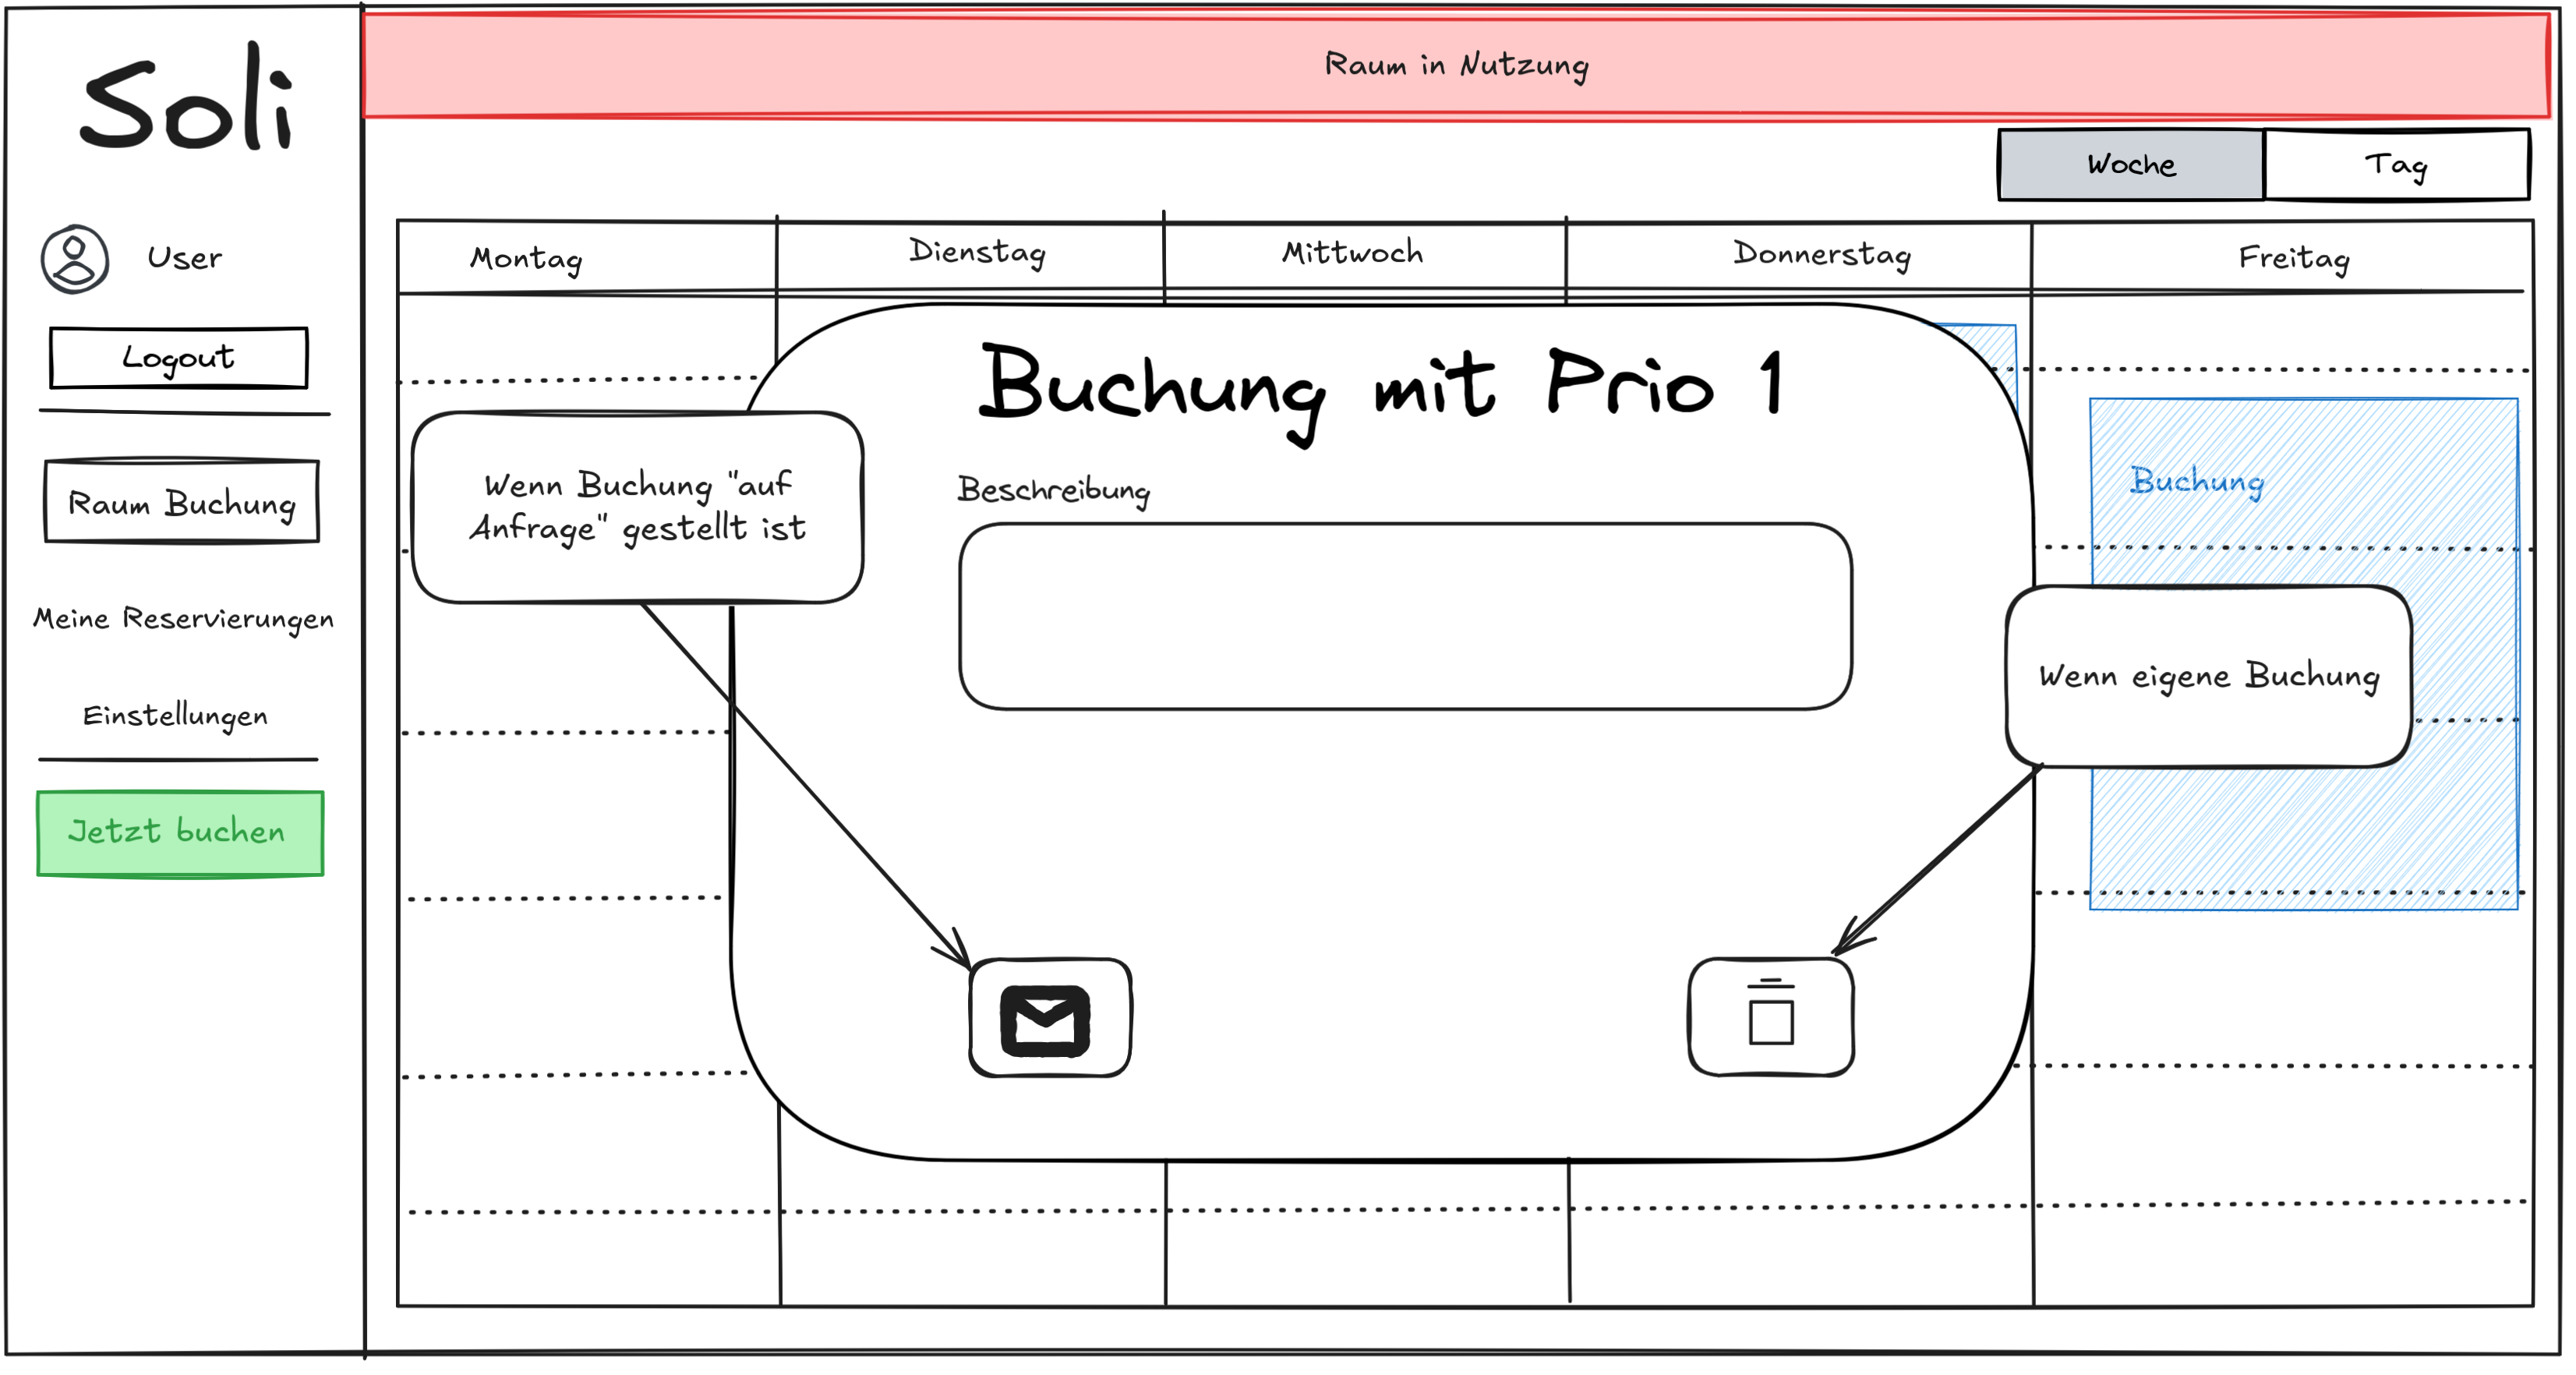
\includegraphics[width=\textwidth]{figures/ui/reservierunginkalendar}
    \caption{Reserverierung im Kalender}
    \label{fig:calendarviewbooking}
\end{figure}
\clearpage

\section{Adminstration}
Ein/e Administrator*in hat die Möglichkeit, über die Benutzeradministrationsoberfläche, die in Abbildung \ref{fig:adminuser} dargestellt ist, Nutzende einzusehen und zu verwalten.

In dieser Ansicht werden alle Nutzenden angezeigt, die sich in der Anwendung registriert haben.
Ein Admin kann die Accounts von Nutzenden deaktivieren und somit ihre Anmeldung verhindern.

Um die Suche nach einem bestimmten Konto zu erleichtern, kann ein Admin nach Kontonamen filtern.

Zudem kann ein Admin die Anmeldung per Gastkonto deaktivieren.
Zweck dieser Funktion ist es, den Missbrauch von Gastkonten z.B.\ durch Bots in vorübergehenden Zeiten zu verhindern.

\begin{figure}[ht]
    \centering
    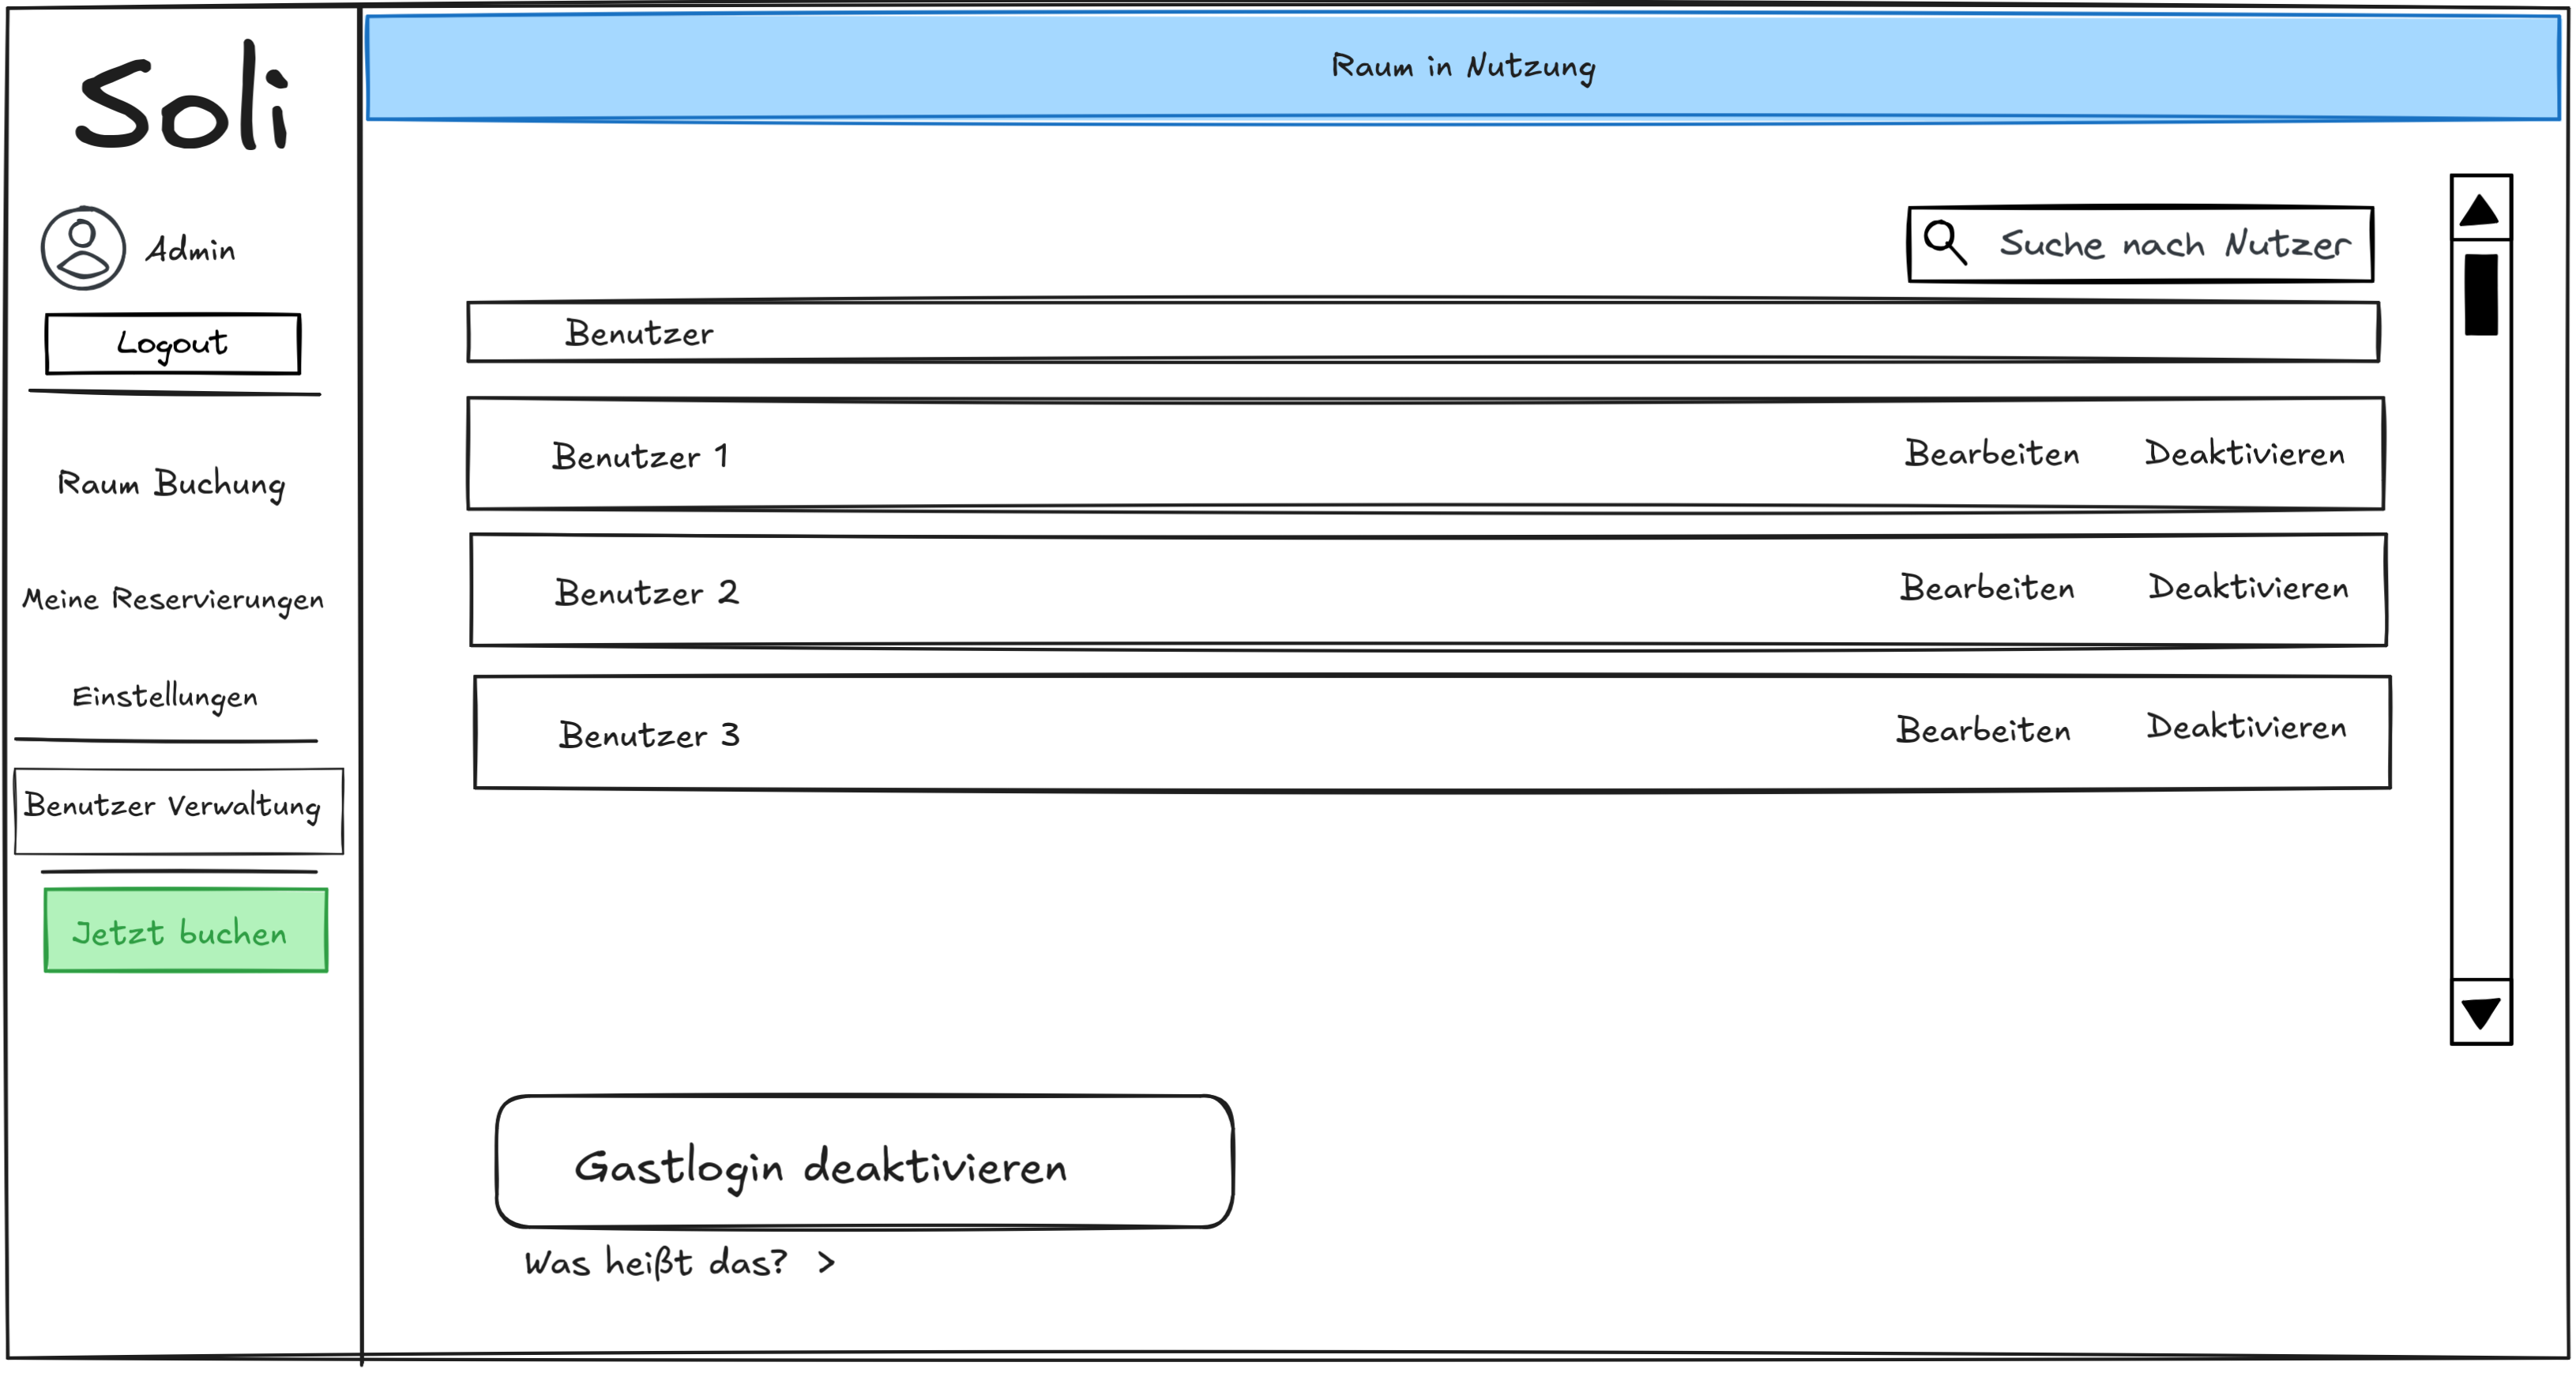
\includegraphics[width=\textwidth]{figures/ui/useradminui}
    \caption{Benutzeradminstrationsoberfläche}
    \label{fig:adminuser}
\end{figure}

